En differensial opamp har signal på begge input.

\begin{figure}[H]
  \caption{Differensial OpAmp}
  \centering
  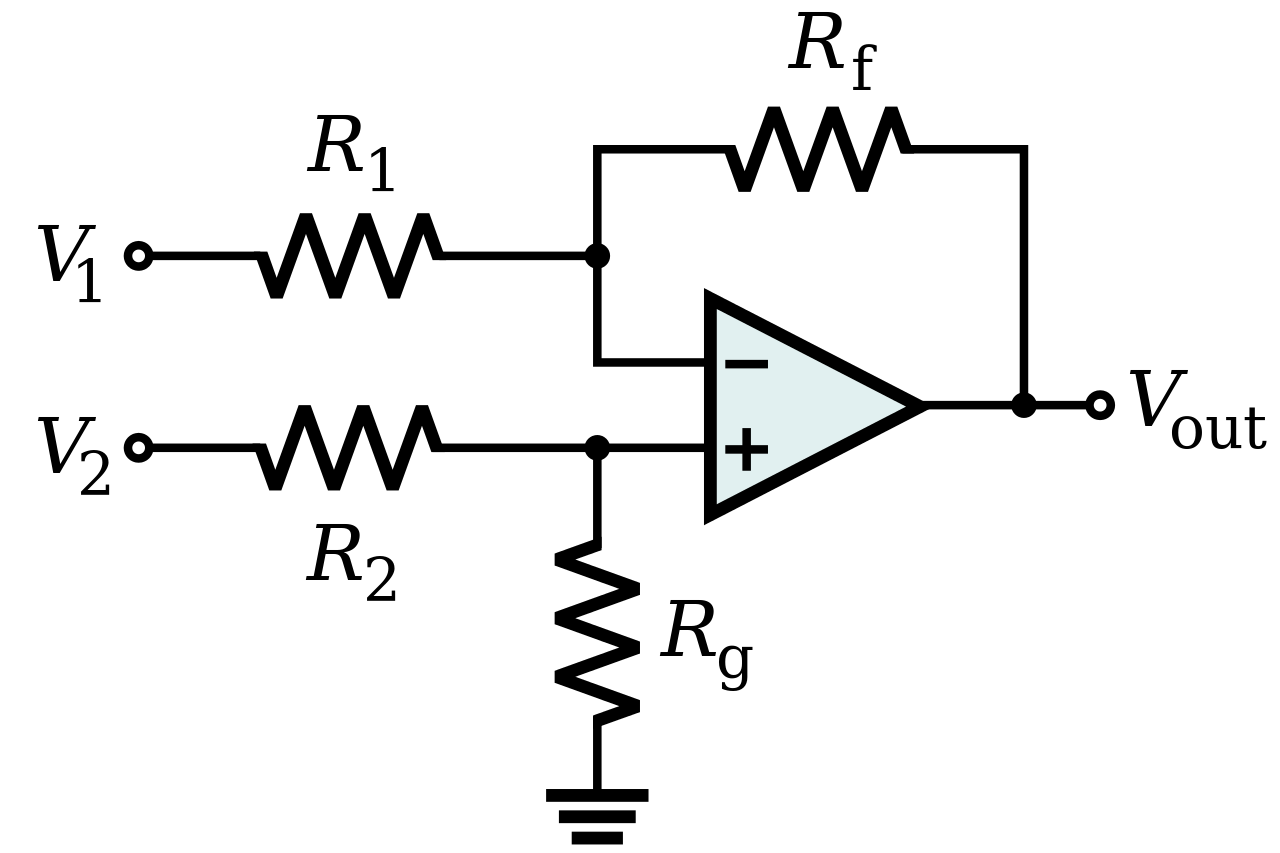
\includegraphics[width=0.5\textwidth]{./img/diffamp}
\end{figure}

For å finne $v_o$ bruker man superposisjonsprinsippet.
\\\\
$v_1$ alene $(v_2 = 0)$
$$v_{o1} = -\frac{R_f}{R_1} \cdot v_1$$

$v_2$ alene $(v_1 = 0)$
$$v_{o2} = \frac{R_f + R_1}{R_1} \cdot v_g$$
$$v_g = \frac{R_g}{R_2 + R_g} \cdot v_2$$
$$v_{o2} = \frac{R_f+R_1}{R_1} \cdot \frac{R_g}{R_2+R_g} \cdot v_2$$

Summen av bidragene
$$v_o = v_{o1} + v_{o2} =
  -\frac{R_f}{R_1}v_1 + \frac{(R_f+R_1)R_g}{R_1(R_2+R_g)}v_2$$
